\documentclass{article}
\usepackage{geometry}
\usepackage{graphicx}
\usepackage{setspace}

% Path to graphic images
% \graphicspath{ }

% Title
\title{Wifi Connected Chess Boards \\ \large Project Requirement Specification}
\author{Nick Kraus, Kyle Jameson, Maurice Wallace, Mark Mauriello}
\date{\today}

% Margins
\geometry{letterpaper, portrait, margin=.75in}

\doublespacing

\begin{document}

\maketitle

%-----------------------
%	Project Overview	
%-----------------------

\section*{Purpose}
\indent

The goal of our project is to create a physical implementation of an internet chess game. The practical purpose is to provide entertainment value to the users by allowing them to play chess against others over the internet with a physical chess set. This project will allow those users to have the best of both sides of internet and board based chess.

\section*{Definitions}
\indent

\begin{itemize}
	
	\item Embedded System: A computer system that is within and controls a larger mechanical or electrical system.
	\item Microcontroller: A small computer with programmable inputs and outputs.
	\item UART: A Universal Asynchronous Receiver Transmitter, a method to serially send data over electrical wires.
	\item Reed Switch: An electrical switch which triggers in the presence of a magnetic field.
	\item Limit Switch: A switch that triggers when an object collides with it.
	\item Gantry: A structure with a moving platform.
	\item Stepper Motor: An electric motor which divides a full rotation into a number of discrete equal steps.
	\item API: An application programming interface, which allows different software systems to interface with each other.
	\item Client Server Architecture: An architecture in which the clients (which run the users application) communicate with each other through a central server.
	\item Bare Metal: A term referring to software that runs directly on a processor without any supporting operating system.

\end{itemize}

\section*{System Overview}
\indent

Our project will have four main systems. These four systems are the electrical system, mechanical system, client software (firmware), and server software. The client software will be the firmware for the electrical system, and therefore control the mechanical system. It will also act as the main application for the user. The server software will allow different clients to communicate with each other.

\subsection*{Electrical System}
\indent

An embedded circuit board will house all of the electrical components, including the microcontrollers which will run the client software, and the WiFi module which will be used to communicate with the server software. The electrical system will measure the state of the chess board through reed switches, and control the mechanical system by using stepper motors and motor drivers. The microcontroller used will be a Cypress CY8C5268AXI ARM Cortex-m3, and it will use two Allegro A4988 stepper motor drivers to control the motors. An array of 96 reed switches will be used to determine if a piece exists on the space above.

\subsection*{Mechanical System}
\indent

The mechanical system will control the movement of pieces on the chess board. It will use an X-Y gantry underneath the playing surface equipped with an electromagnet to move the pieces. The electrical system will be used to monitor and drive the mechanics to make sure they are operating properly. The gantry will be driven in an h-bot configuration by two stepper motors. The stepper motors work together to drive the gantry in an axis, by driving a GT2 timing belt connected to the gantry and some bearings around the frame. The electromagnet which will move the pieces will be raised and lowered by a small servo and turned on and off using a large power mosfet.

\subsection*{Client Software}
\indent

The client software is the bare metal firmware which runs the user facing application as well as controls all of the mechanical system. It is written in the C programming language, using libraries and APIs provided by Cypress for its line of ARM microcontrollers and by the open source community surround the ESP8266 and Arduino. The Cypress libraries abstract away accessing registers used to write to GPIO pins as well as timing for the LCD displays and UART bus, as well as provide simple functions with which to interact with these peripherals. It consists of code for an ARM microcontroller and the ESP8266 WiFi module, which communicate with each other over a UART serial bus. The microcontroller will implement many high level functions to interact with the underlying mechanical hardware, the web server, and the user interface. To interact with the mechanical system a MoveGantry() function will be used to move the underlying gantry by a set measurement. To help make sure this is always correctly calibrated a Home() function will be implemented which brings the gantry back to the (0, 0) position, as defined by hardware switches. There will be a SetMagnet() function which allows you to turn the magnet for moving chess pieces on or off, and a ScanBoard() function which reads which squares have a piece over them. We will also use high level C functions as the basis for our algorithms necessary for our project. There will be an IsLegal() function which determines if the last play was a legal chess move, a MovePiece() function which will find a possible set of moves for a chess piece without hitting any others on the board, and a IsCheckmate() function which determines if the current state is a checkmate for one of the players.

\subsection*{Server Software}
\indent

The server software allows one chess board to communicate with another. It offers an API as an interface for the WiFi module to communicate with, and provides a central location for the chess boards to connect to. The server will host an HTML webpage through python which will respond to HTTP GET and POST requests to send the current state of the board to the other board, at the end of each turn. It will have a SQL database on the back-end that stores the state of the game after each turn, and then sends it to the opposing board to move accordingly.

\begin{figure}
    \centering
    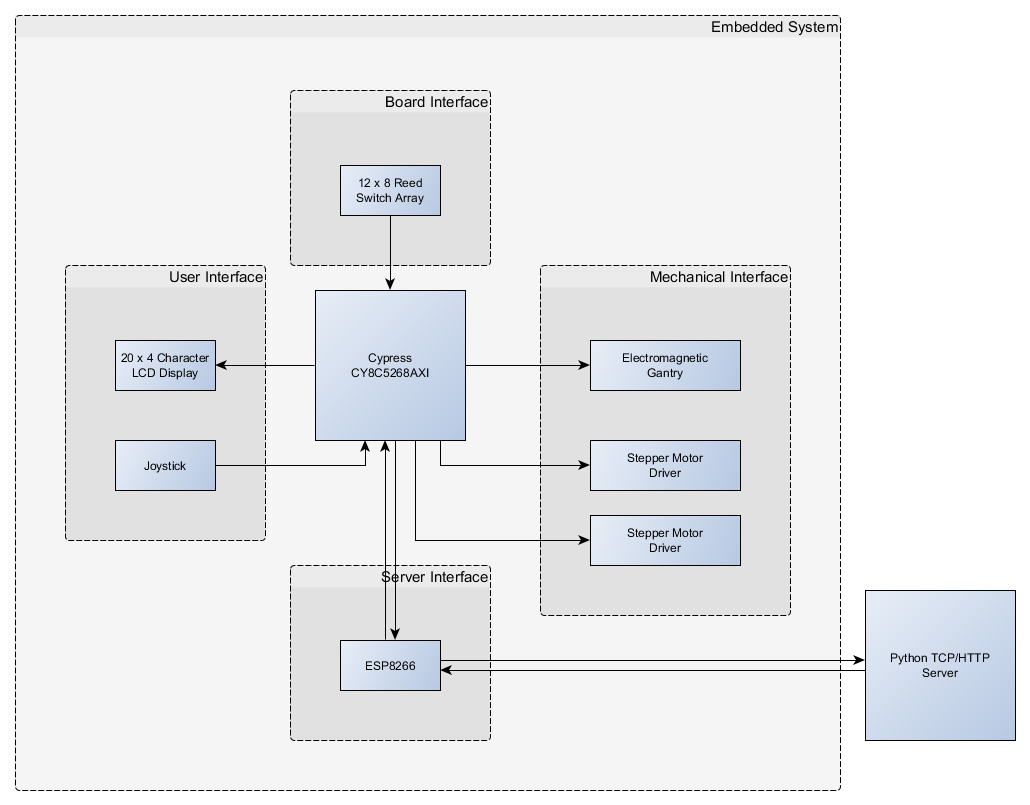
\includegraphics[scale=0.5]{BlockDiagram}
    \caption{Diagram of the WiFi chessboard embedded system.}
\end{figure}

%--------------------------
%	Project Description	
%--------------------------

\section*{Project Features}

\begin{itemize}

	%Basic

	\item Board State: Be able to read all chess positions to determine whether a piece is at that position or not. (Basic)
	\item Opponent Connection: Be able to connect to an opponent board in order initiate the start of a chess game. (Basic)
	\item Opponent Communication: Communicating the current state of one board to the other to advance the game a turn. (Basic)
	\item Move Recognition: Recognize moves and only allow valid chess moves to be sent to opponent. (Basic)
	\item State Interaction: Have the chess board react to an opponents game state by relocating pieces to their correct position. (Basic)
	\item Game Completion: Implement a way to signal that a game of chess has been completed. (Basic)
	\item Piece Graveyard: A dedicated area for each piece to go when taken out of the game. (Basic)
	\item Error Notification: If an error occurs during any point in the gameplay error codes can be sent to the LCD screen so that the user can troubleshoot the problem or reset the board to continue gameplay. (Basic)

	%Desired

	\item Virtual Interface: Allow a computer program to play a game of chess against the physical board. (Desired)
	\item Checkmate Detection: Detect if a checkmate has occurred and signal end of game if so. (Desired)
	\item Stalemate Detection: Detect whether a stalemate occurred and signal end of game if so. (Desired)
	\item Game Resume: Continue a previously played chess game from a predetermined starting point. (Desired)
	\item State Recording: Record all states of a chess game as its played. (Desired)
	\item Chess Timers: Include move timer and different variations of how they're used. (Desired)

	%Dream

	\item Arbitrary Positioning: Be able to relocate any correct board set up to any other correct one. (Dream)
	\item Chess Variants: Be able to play chess variations with all rules implemented by the system. (Dream)
	\item AI: Server side AI for playing against an artificial opponent. (Dream)
	\item Game Playback: Play through all moves of a recorded chess game. (Dream)
	\item Standardized Recording: Record all game moves in a standardized chess move format. (Dream)

\end{itemize}

\section*{System Interfaces}

\subsubsection*{User Interfaces}
\indent

This project will have two separate parts to its user interface, the actual chess board itself and a LCD screen with tactile buttons. The chess board and pieces will allow the user to control the state of the chess game, just like in a physical version of the game; moving a piece will move that equivalent piece on the opponents board. The LCD and buttons will allow the user to modify stages and options within the game, such as marking the end of a turn or setting up a new game with another player. To interface the hardware with the user interface some high level C functions are going to be used. An LCDWrite() function will clear the display and then write a string to it, allowing text to be displayed from the microcontroller to the user, and a ButtonRequestHandler() function will be set up to an interrupt and called every time a UI button is pressed. From this we can then set the correct functionality depending on the button pressed.

\subsubsection*{Hardware Interfaces}
\indent

The client software is firmware for the microcontrollers that make up the embedded system. These microcontrollers will be used to get user input and control the mechanical system. The microcontrollers have programmable inputs and outputs which will allow us to get the state of the chess board, control the stepper motors and electromagnet that will move the pieces, drive displays and button arrays for the user input, and communicate over a WiFi network. The stepper motors are driven using a step/dir interface where a pulse is put on the step pin, and depending on the value of the dir pin the motor will move either clockwise or counter-clockwise. A microcontroller pin will be used to drive a FET which will turn on the electromagnet and raise it to the surface with a servo.

\subsubsection*{Software Interfaces}
\indent

This project will have two sets of software that will interface with each other: the client software and the server software. The client software will connect to the server through a TCP connection and use the API that the server exposes to set up games with other players and communicate the game state to the opponents board.

\subsubsection*{Communication Interfaces}
\indent

Communication in this project is split up between communication in the embedded system and communication that connects the client to the server. To connect the client to the server a TCP connection will be used over a WiFi network. This connection will allow the client to reliably connect to the server, and make sure that no packets are lost during data transfers. The server will run an HTTP server using python, and the firmware on the microcontroller will interact to the server through the ESP8266 module. The microcontroller will contain functions such as WiFIStart() which will start the wifi module, connect it to the server and send a handshake packet to make sure communications are working. There will also be a WiFiSendState() and WiFiReadState() function which will send and receive the state of the game at the end of each turn. These will be sent as HTTP GET and POST requests to the server at a certain address, which will then respond accordingly. The embedded system will be interconnected using UART buses. These will allow any microcontrollers to communicate with each other and allow the WiFi module to connect to the microcontrollers.

\subsubsection*{Dependencies}
\indent

Either a web server or a software interface to an existing chess server will be required for this project to operate correctly. The platforms this will run on are yet to be determined, but there are many choices such as running a local server, using an existing server architecture like Amazon Web Services, or using the existing chess servers at freechess.org.

\end{document}